\documentclass[10pt,a4paper,twocolumn,twoside]{article}
\usepackage[utf8]{inputenc}
\usepackage[catalan]{babel}
\usepackage{multicol}
\usepackage{graphicx}
\usepackage{fancyhdr}
\usepackage{times}
\usepackage{titlesec}
\usepackage{multirow}
\usepackage{xurl}
\usepackage[hidelinks,breaklinks=true]{hyperref}
\usepackage[top=2.5cm, bottom=1.3cm, left=1.2cm, right=1.2cm]{geometry}
\usepackage[figurename=Fig.,tablename=Taula,font={small,sf}]{caption}
%\usepackage[font={small,sf}]{caption}

\raggedbottom

\usepackage{enumitem}
\setlist[itemize]{noitemsep}
\setlist[enumerate]{noitemsep}

\let\OLDthebibliography\thebibliography
\renewcommand\thebibliography[1]{
  \OLDthebibliography{#1}
  \setlength{\parskip}{0pt}
  \setlength{\itemsep}{0pt plus 0.3ex}
	\sloppy
	\raggedright
	\emergencystretch=2em
}

\pagestyle{fancy}
\fancyhf{}
\fancyhead[LO]{\textsf{\small $\mu$Projecte VC(GEI)-PSIV(GED), Escola d’Enginyeria (EE), Universitat Autònoma de Barcelona (UAB)}}
\fancyhead[RE]{\textsf{\small $\mu$Projecte VC(GEI)-PSIV(GED), Escola d’Enginyeria (EE), Universitat Autònoma de Barcelona (UAB)}}
\renewcommand{\headrulewidth}{0pt}

\titleformat*{\section}{\large\sffamily\scshape\bfseries}
\titleformat*{\subsection}{\normalsize\sffamily\bfseries}
\titleformat*{\subsubsection}{\normalsize\sffamily\slshape}

\begin{document}

{\sffamily
% Titol
\noindent\textbf{\LARGE Detección de gestos y lengua de signos}
% autors
\begin{center}
Alfons Baiges, Héctor Berger, Gonzalo Maurín
\end{center}

\bigskip
\bigskip

\noindent 
\textbf{Abstract}--- Lorem ipsum dolor sit amet, consectetur adipiscing elit. Curabitur quis fermentum orci. Aliquam sodales varius blandit. Vestibulum congue tortor a fringilla venenatis. Nam magna ex, fringilla eu porta facilisis, consequat quis orci. Vivamus ut mattis metus. Interdum et malesuada fames ac ante ipsum primis in faucibus. Maecenas a orci at nibh so-dales condimentum. Orci varius natoque penatibus et mag-nis dis parturient montes, nascetur ridiculus mus. 


Duis interdum nisi id sem dictum rhoncus. Duis vitae ante tincidunt, tempor diam quis, tincidunt lorem. Etiam sit amet nisi tempus sapien auctor vestibulum ac eu purus. Curabi-tur a suscipit urna, sit amet facilisis erat. Morbi iaculis ves-tibulum tortor, quis varius justo mollis ut. Pellentesque plac-erat felis pretium, maximus ex quis, rutrum nisi. Sed quis imperdiet nunc. Donec euismod ipsum sed urna semper posuere. Nunc id gravida enim. Suspendisse tortor lectus, tempus tincidunt tellus at, mattis tincidunt tortor. Morbi fini-bus ultrices bibendum. Morbi ac ipsum eu erat consectetur convallis at. 

\bigskip

\noindent 
\textbf{Keywords}---Visión por Computador, Reconocimiento de Gestos, Deeplearning, OTSU \& canny edge detection, Lengua de signos ASL MNIST, Skeleton-Based Dynamic Hand Gesture Recognition.
}
\bigskip

{\vrule depth 0pt height 0.5pt width 3cm\hspace{7.5pt}%
\raisebox{-3.5pt}{\fontfamily{pzd}\fontencoding{U}\fontseries{m}\fontshape{n}\fontsize{11}{12}\selectfont\char70}%
\hspace{7.5pt}\vrule depth 0pt height 0.5pt width 3cm\relax}

\bigskip


\section{Introducción}

El reconocimiento de gestos es un campo muy importante dentro de la visión por computador, 
con variedad de aplicaciones entre humano-ordenador, accesibilidad y sistemas de comunicación no verbal. 
Nos centraremos en la interpretación del lenguaje de señas y el análisis de gestos en tiempo real para realizar comandos en una aplicación. 
Para ello nos hemos planteado cuatro etapas diferentes por las cuales iremos evolucionando progresivamente desde métodos clásicos hasta un modelo de aprendizaje profundo. 

\begin{itemize} %equivalències aproximades en word
\item	Reconocimiento de manos: En la fase incial nuestro objetivo principal es la detección de manos sin ningún significado concreto, solo para poder ser capaces de diferenciar manos del resto de la imagen con técnicas clásicas.
\item	Detección de gestos: en esta etapa nos fijaremos en como detectar gestos concretos, con técnicas como Harris y LBP/HOG.
\item	Detección con Deep Learning: continuaremos esta vez con una detección de señas en ASL (American Sign Language), ya que hemos encontrado un dataset MNIST preprocesado.
\item	Detección de gestos con aprendizaje profundo y información esqueletal: finalmente, utilizaremos un dataset de gestos (tanto propio como externo) para entrenar un modelo de gestos dinámicos. Además de programar comandos sencillos en un programa para realizarlos en tiempo real.
\end{itemize}

\section{Objetivos}

El objetivo principal de este proyecto es desarrollar y evaluar diferentes métodos de reconocimiento de manos, gestos y lengua de signos mediante técnicas de visión por computador clásica y modelos de aprendizaje profundo.

El proyecto se estructura en tres líneas principales de trabajo: detección clásica de manos en imágenes, reconocimiento de gestos estáticos mediante características visuales y clasificación de signos mediante redes neuronales, incluyendo también el uso de información esqueletal para gestos de mano.

Para alcanzar este objetivo general, se plantean los siguientes objetivos:

\begin{itemize}
\item Implementar un sistema clásico de segmentación de manos mediante diferencia con el fondo, detección de piel en YCrCb, operaciones morfológicas y componentes conectados.

\item Detectar y analizar gestos estáticos como thumbs up, thumbs down, palm y ok mediante contornos, centroides, convex hull y descriptores ORB.

\item Entrenar una red neuronal convolucional sobre el dataset ASL MNIST para clasificar letras del lenguaje de signos americano, aplicando técnicas de data augmentation.

\item Implementar un sistema de predicción capaz de cargar un modelo entrenado y clasificar imágenes externas de signos.

\item Entrenar y evaluar un modelo de Deep Learning basado en información esqueletal de la mano.

\item Evaluar los resultados mediante métricas como accuracy, loss, matriz de confusión y reporte de clasificación.
\end{itemize}

Como criterio de éxito, se espera obtener una segmentación visualmente correcta de la mano en imágenes con fondo controlado, una comparación razonable entre gestos estáticos mediante descriptores visuales y una precisión elevada en los modelos de clasificación basados en Deep Learning.
\section{Estado del arte}

El campo del reconocimiento de movimiento de manos se encuentra hoy en día en un estado muy avanzado, con una amplia variedad de estrategias y enfoques para abordar este problema. A lo largo del tiempo, estas técnicas han experimentado una evolución significativa, pasando de métodos más simples y limitados, basados en reglas y sensores físicos, a enfoques mucho más sofisticados. En la actualidad, destacan especialmente las soluciones basadas en Deep Learning, que permiten analizar grandes volúmenes de datos y captar patrones complejos con gran precisión, mejorando notablemente el rendimiento y la adaptabilidad de estos sistemas en diferentes aplicaciones. 

Técnicas que consideramos más importantes: 

\subsection{Apartado fisico}

Uso de algún elemento físico para facilitar el reconocimiento de la mano
\begin{itemize}
\item	Guante: utiliza un guante con sensores para capturar el movimiento de la mano y la posición la palma y los dedos para poder la extremidad. Esta opción tiene la limitación de que es necesaria una conexión física con el ordenador que se este utilizando para la lectura de datos. 
\item	Color: detectan la piel mediante modelos de color o utilizan marcadores de colores específicos para identificar la mano dentro de la imagen. Estos métodos se basan generalmente en la segmentación por color, ya sea en espacios como RGB, HSV o YCbCr, lo que permite aislar regiones que coinciden con tonos de piel o con colores previamente definidos para los marcadores. Gracias a su simplicidad, son fáciles de implementar y requieren un bajo coste computacional, lo que los hace adecuados para aplicaciones en tiempo real o sistemas con recursos limitados. 
\end{itemize}

\subsection{Apartado digital}
\begin{itemize}
\item	Esqueleto: extraen puntos clave de la mano y de sus articulaciones, lo que permite representar de manera estructurada la posición y el movimiento de cada dedo y de la palma. Estos puntos, facilitan la construcción de un modelo geométrico de la mano que resulta especialmente útil para expresar y analizar gestos de forma precisa. A partir de esta información, es posible calcular características relevantes como la orientación de las articulaciones, la distancia entre puntos clave, los ángulos formados entre los dedos y las trayectorias de movimiento. Estas propiedades permiten capturar tanto la forma estática de la mano como su dinámica en el tiempo, lo que mejora significativamente la capacidad de los sistemas para reconocer gestos complejos. 
\item	Apariencia: analizan la forma visual de la mano a partir de características extraídas directamente de la imagen, como la detección de bordes, contornos y siluetas. Estos métodos se centran en la información global de la mano, capturando su forma y estructura sin necesidad de modelos internos complejos. Gracias a ello, suelen ser eficientes computacionalmente y funcionan bien en tiempo real, lo que los hace adecuados para aplicaciones interactivas. 
\item	Movimiento: detectan gestos a partir de cambios en los fotogramas, son útiles para gestos dinámicos con un fondo estable, pero si el fondo es en movimiento son incapaces de detectarlo. Este enfoque permite identificar la dinámica del gesto, es decir, cómo se desplaza la mano a lo largo del tiempo, lo que resulta especialmente útil para reconocer gestos dinámicos que implican trayectorias o movimientos continuos. 
\item	Profundidad: usan cámaras específicas para obtener información 3D, mejoran la segmentación pero es necesario el hardware especifico. Con este método se puede conseguir información como la distancia entre mano y cámara, lo que permite una la mejora de segmentación. 
\item	Modelos 3D: buscan reconstruir la pose completa de la mano en el espacio tridimensional, teniendo en cuenta la posición y orientación de dedos y articulaciones, gracias a esto permiten una representación más precisa y detallada del gesto, sin embargo, son más complejos computacionalmente y muchos de ellos necesitan de sensores adicionales (cámaras de profundidad...). 
\end{itemize}

\subsection{Uso de redes neuronales}
\begin{itemize}
\item	Deep Learning: los modelos basados en deeplearning usan redes neuronales, especialmente redes neuronales convolucionales (CNN) para aprender automáticamente representaciones relevantes a partir de los daos de entrada, eliminando la necesidad de diseñar manualmente las características. Estos modelos son actualmente superiores en cuanto al reconocimiento de gestos, tanto en imágenes como video, gracias a su capacidad para capturar patrones espaciales y, en casos, temporales. Sin embargo, estos métodos requieres grandes volúmenes de datos etiquetados para su entrenamiento, asi como un elevado coste computacional, lo que puede dificultar su implementación. 
\end{itemize}

\section{Propuesta}
El material que vamos a utilizar para realizar nuestros experimentos se basa en dos datasets de \emph{kaggle}, y un pequeño dataset creado a partir de unos videos grabados por nosotros. Haremos Data Augmentation en este último. 

\subsection{ASL MNIST}
El primer dataset que usaremos es el MNIST (por sus siglas en inglés, Modified National Institute of Standards and Technology database) no oficial del alfabeto del lenguaje de señas americano \cite{dataset_MNIST_ASL}. 

El Lenguaje de Señas MNIST se encuentra en formato Formato CSV, con etiquetas y valores de píxeles en filas individuales. Cada fila es una imagen en escala de grises de una mano haciendo un gesto.  
Este base de datos representa 24 clases de letras (excluyendo J y Z que requieren movimiento). Por lo tanto, cada caso representa una etiqueta (0-25) como un mapa 1-1 para cada letra del alfabeto A-Z (sin 9=J ni 25=Z).
Tenemos 27.455 casos de entreno y 7172 casos para test, susceptible a modificaciones. 

\subsection{Información Esqueletal}
El segundo dataset de \emph{kaggle} \cite{dataset_Multi-Modal} se divide en dos ya que es multi-modal, en imagenes de gestos con las manos: cercanas al infrarojo y información esqueletal. Nos parecen más relevantes el segundo tipo de datos, ya que es una técnica más actualizada y interesante sobre la que trabajar. Este dataset son realmente 15 gestos diferentes (palma hacia arriba, números, pulgar arriba, etc), 6 veces cada, de 15 sujetos diferentes (5 mujeres y 10 hombres). 
Tenemos $15*15*200=45000$ casos para entrenar y testear nuestro modelo. 

\subsection{Dataset Propio}
Construiremos un dataset propio a partir de videos captados con la webcam integrada en nuestos portátiles. Nos centraremos en 5 gestos con movimiento para realizar 5 comandos diferentes, recopilaremos estos datos con información esqueletal como en el anterior dataset pero quedandonos con los principales atributos necesarios. 
La idea es crear 75 casos reales, 25 gestos (5 de cada tipo) por cada integrante del grupo, posteriormente a partir de recortes y giros aumentar el volumen a mínimo 250 casos. 


\section{Experimentos, resultados y análisis}

A continuación vamos a detallar los diferentes experimentos y sus correspondientes analisis de cada fase.

\subsection{Primera etapa: Técnicas clásicas}

Para empezar hemos querido utilizar algunas de las técnicas aprendidas en clase de Procesacmiento de Sonido, Imagen y Vídeo. 
Al inicio hemos trabajado con una sola imagen, para trabajar bien sobre la segmentación de una mano.

Para ello, hemos utilizado imagenes capturadas con nosotros mismos, con un fondo controlado y con la mano en primer plano. Haciendo gestos simples como thumbs up, thumbs down, palm y ok.
En primer lugar, se aplica detección de cambio respecto a una imagen de fondo vacío utilizando la diferencia absoluta entre imágenes. Esto permite identificar únicamente las regiones que contienen movimiento o nuevos objetos en escena. Posteriormente, la imagen se transforma al espacio de color YCrCb, donde se aplica una segmentación de piel mediante umbralización sobre los canales Cr y Cb.
Una vez obtenidas ambas máscaras binarias, se combinan utilizando operaciones lógicas para conservar únicamente las regiones que corresponden simultáneamente a cambios respecto al fondo y colores compatibles con piel humana. Para mejorar la calidad de la segmentación, se aplican operaciones morfológicas como apertura, cierre y dilatación, eliminando ruido y pequeñas regiones no relevantes.
Después del preprocesado, se utilizan componentes conectados para filtrar regiones pequeñas y conservar únicamente las zonas con mayor probabilidad de corresponder a la mano. Finalmente, se extraen los contornos de la región segmentada y se representan sobre la imagen original para visualizar el resultado de la detección.
Además de la segmentación, se implementaron técnicas básicas de análisis geométrico de la mano. Mediante convex hull y defectos de convexidad se estimó el número aproximado de dedos levantados. También se utilizaron descriptores ORB para detectar puntos clave y comparar distintos gestos a partir de la similitud entre descriptores visuales.
Esta primera etapa permitió comprender el funcionamiento de técnicas clásicas de procesamiento de imagen y establecer una base sólida antes de avanzar hacia métodos basados en Deep Learning.

Además de la segmentación clásica, en esta etapa también se estudiaron diferentes métodos de extracción de características para describir y comparar gestos de la mano. Para ello, se utilizaron descriptores locales ORB Oriented FAST and Rotated BRIEF, capaces de detectar puntos clave invariantes a rotación y pequeños cambios de escala.
A partir de las regiones segmentadas de la mano, se extrajeron puntos de interés y descriptores visuales asociados a cada gesto. Posteriormente, estos descriptores se compararon mediante Brute Force Matching, evaluando el número de coincidencias entre diferentes imágenes de gestos. Esto permitió analizar la similitud entre gestos estáticos y estudiar la capacidad de los descriptores para diferenciar configuraciones distintas de la mano.
Esta fase permitió combinar técnicas clásicas de segmentación y análisis de características locales, estableciendo una transición natural hacia métodos de reconocimiento más avanzados basados en aprendizaje profundo.

\subsection{Segunda etapa: Deep Learning ASL MNIST}
En esta segunda etapa hemos virado en las tecnicas usadas, pasando de las clasicas de la anterior fase al Deep learning. Para eso hemos utilizado una base de datos que consiste de todas las letras del alfabeto en American Sing Language (ASL), menos dos, la j y l z, las cuales requiren de movimiento y para esta etapa hemos utilizado únicamente imagenes. Realmente el dataset no contenia imagenes si no directamente unos vectores que representan todos los pixeles de la imagen 28x28, 764 en total. Además, el dataset ya viene separado entre la parte de train y la de test
El modelo emplea una estructura secuencial diseñada para la extracción jerárquica de rasgos. Comienza con dos bloques de convolución y MaxPooling (32 filtros de 3x3 y luego 64 filtros); estos se encargan de detectar desde bordes básicos hasta formas complejas de la mano.

Tras la extracción, una capa Flatten convierte los mapas bidimensionales en un vector para la fase de clasificación. Esta etapa final utiliza capas densas de 128 y 256 neuronas con activación ReLU, reforzadas con capas de Dropout al 30 porciento para prevenir el sobreajuste. El modelo concluye con una capa Softmax de 25 neuronas, que genera la probabilidad final para cada una de las letras del alfabeto ASL procesadas.
Una vez entrenado el modelo, se implementó un sistema de predicción capaz de cargar el modelo entrenado y clasificar imágenes externas de signos. Para ello, se desarrolló una función que recibe una imagen de entrada, la preprocesa de la misma forma que las imágenes del dataset (redimensionado, normalización, etc.) y posteriormente utiliza el modelo para predecir la clase correspondiente al gesto representado en la imagen.
La salida del modelo consiste en una distribución de probabilidades sobre las distintas letras del alfabeto ASL, seleccionándose finalmente la clase con mayor probabilidad como resultado de la predicción.
Esta funcionalidad permite evaluar el rendimiento del modelo sobre datos no vistos durante el entrenamiento y proporciona una herramienta práctica para la clasificación automática de signos en aplicaciones interactivas o en tiempo real.
\subsection{Tercera etapa: Deep Learning Skeletal Information}

En la tercera etapa nos hemos centrado en usar el dataset multimodal, que contiene un dataset con información esqueletal. 

La información esqueletal en visión por computador constituye una representación simplificada del cuerpo humano mediante una estructura de grafos, 
compuesta por nodos que identifican las articulaciones principales (keypoints) y aristas que modelan los segmentos óseos. 
Esta técnica, central en las tareas de estimación de pose (pose estimation), permite transformar datos volumétricos o bidimensionales complejos en una descripción geométrica de baja dimensionalidad. 

Al centrarse exclusivamente en la configuración espacial y la dinámica del movimiento, el análisis esqueletal facilita la extracción de patrones cinemáticos mientras se mantiene la invarianza frente a factores externos irrelevantes, 
tales como la textura de la vestimenta, las condiciones de iluminación o el fondo de la escena. Por ello, es una herramienta fundamental en áreas que requieren una comprensión profunda de la actividad humana, desde el reconocimiento de acciones y el análisis 
biomecánico hasta la interacción persona-computador en tiempo real.

La integración de la información esqueletal es determinante en el reconocimiento de gestos manuales mediante Deep Learning, ya que permite mitigar la complejidad inherente a la alta dimensionalidad 
y a las constantes auto-oclusiones de la mano (como hemos visto en la fase 1). Al abstraer la morfología manual a un conjunto reducido de puntos clave, los modelos logran una invarianza robusta frente a factores extrínsecos como el tono de piel, 
las condiciones de iluminación o la textura del fondo, 
centrando el aprendizaje exclusivamente en la configuración geométrica y cinemática. 
Esta simplificación no solo optimiza drásticamente la eficiencia computacional para el procesamiento en tiempo real, 
sino que también facilita el uso de arquitecturas avanzadas, como las Redes Convolucionales, que explota los datos complejos que serian muy dificiles de extraer con solo pixeles.

Así pues, hemos entrenado un modelo de aprendizaje profundo, una red neuronal densa de 56 → 128 → 64 → 32 neuronas creando un embudo de características cada vez más abstractas.

El dataset se construye mediante procesamiento en paralelo de archivos XML. Se cachea en disco para evitar reprocesamiento innecesario.

De cada muestra se extraen las siguientes características:

\begin{itemize}
	\item Centro de la mano (3D: x, y, z)
	\item Posición de la muñeca (opcional, según disponibilidad)
	\item Para cada dedo (pulgar, índice, corazón, anular, meñique):
	\begin{itemize}
		\item Posición de la punta (3 coordenadas)
		\item Posición MCP - articulación base (3 coordenadas)
	\end{itemize}
	\item Confianza de la detección
	\item GrabStrength y PinchStrength (fuerzas de agarre y pinza)
	\item Indicador de extensión para cada dedo
\end{itemize}


Los datos se dividen en 80\% entrenamiento y 20\% test, y se normalizan respectivamente.

Los resultados obtenidos de nuestro experimento son los siguientes para 50 epochs: 

\begin{figure}[!ht]
\centering
	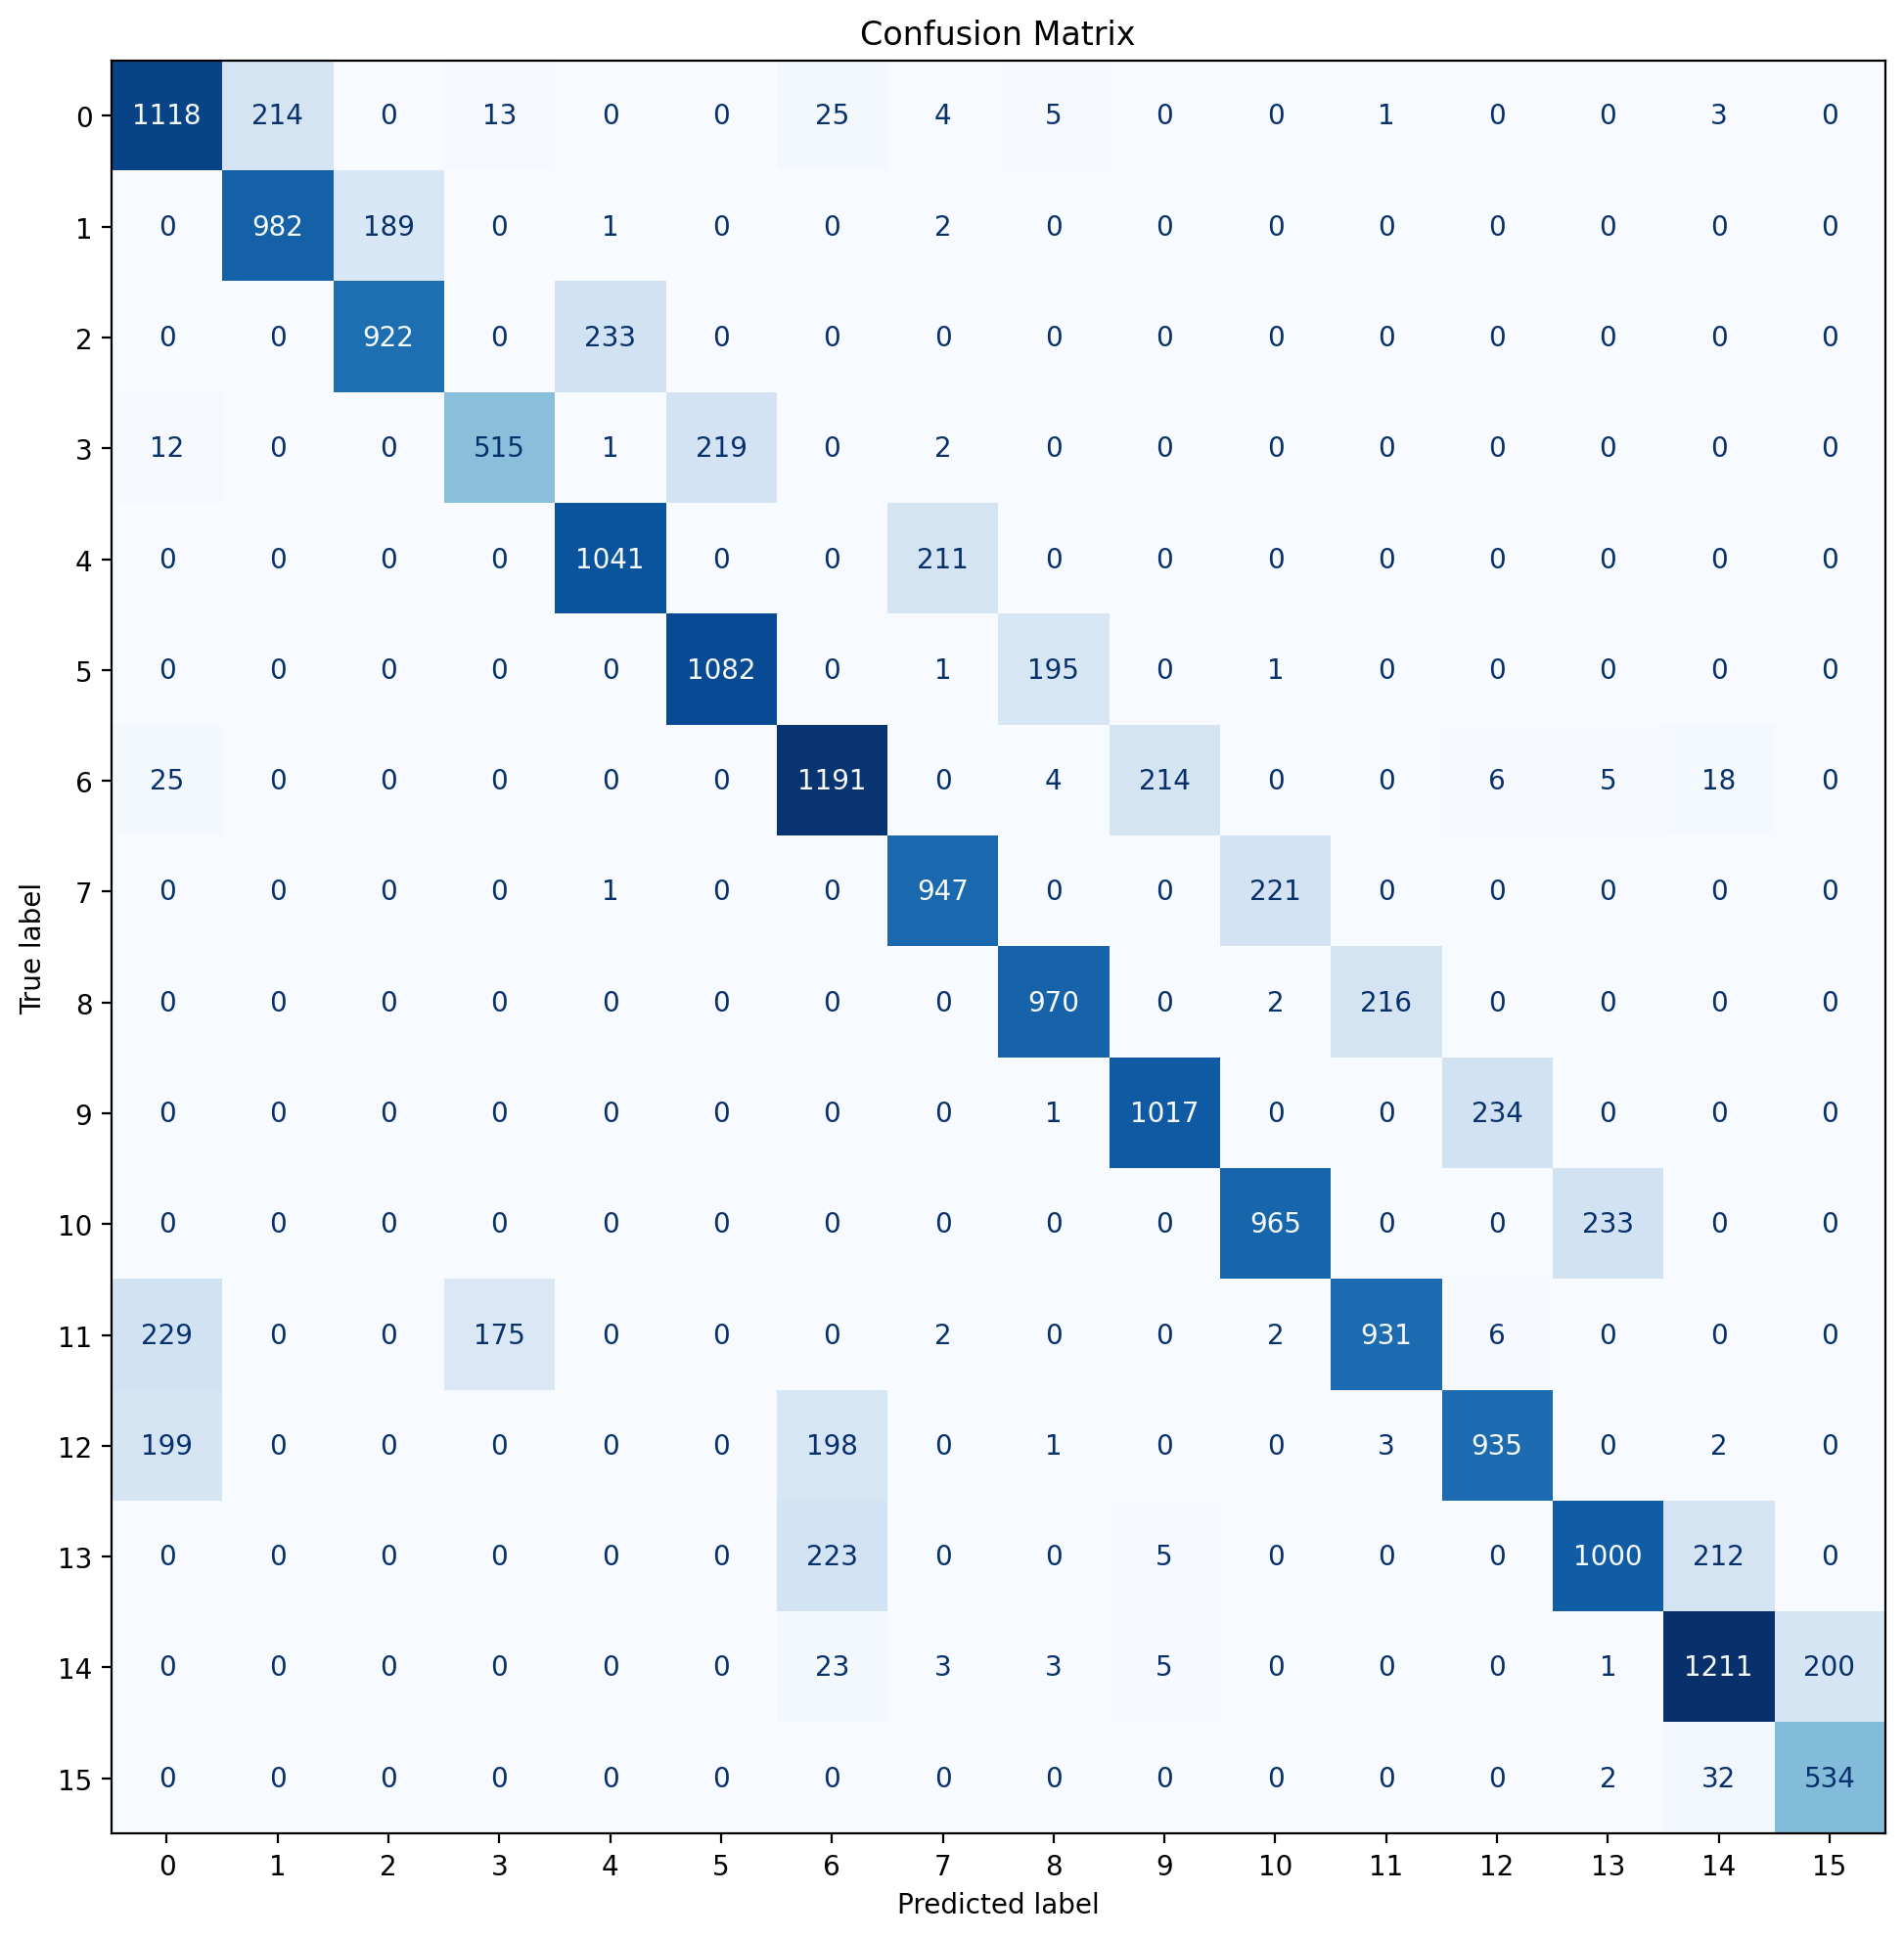
\includegraphics[width=0.4\textwidth]{figs/confusion_matrix.png}
	\caption{Matriz de confusión.}
	\label{f:detall}
\end{figure}



Actualmente hemos alcanzado un 78\% de precisión con el modelo actual, bastante bueno pero con margen de mejora.
Podemos analizar la evolución de la precisión con la siguiente figura:
% Per a fer que la figura ocupi les dues columnes utilitzeu "figure*" per comptes de "figure"
\begin{figure}[!ht]
\centering
	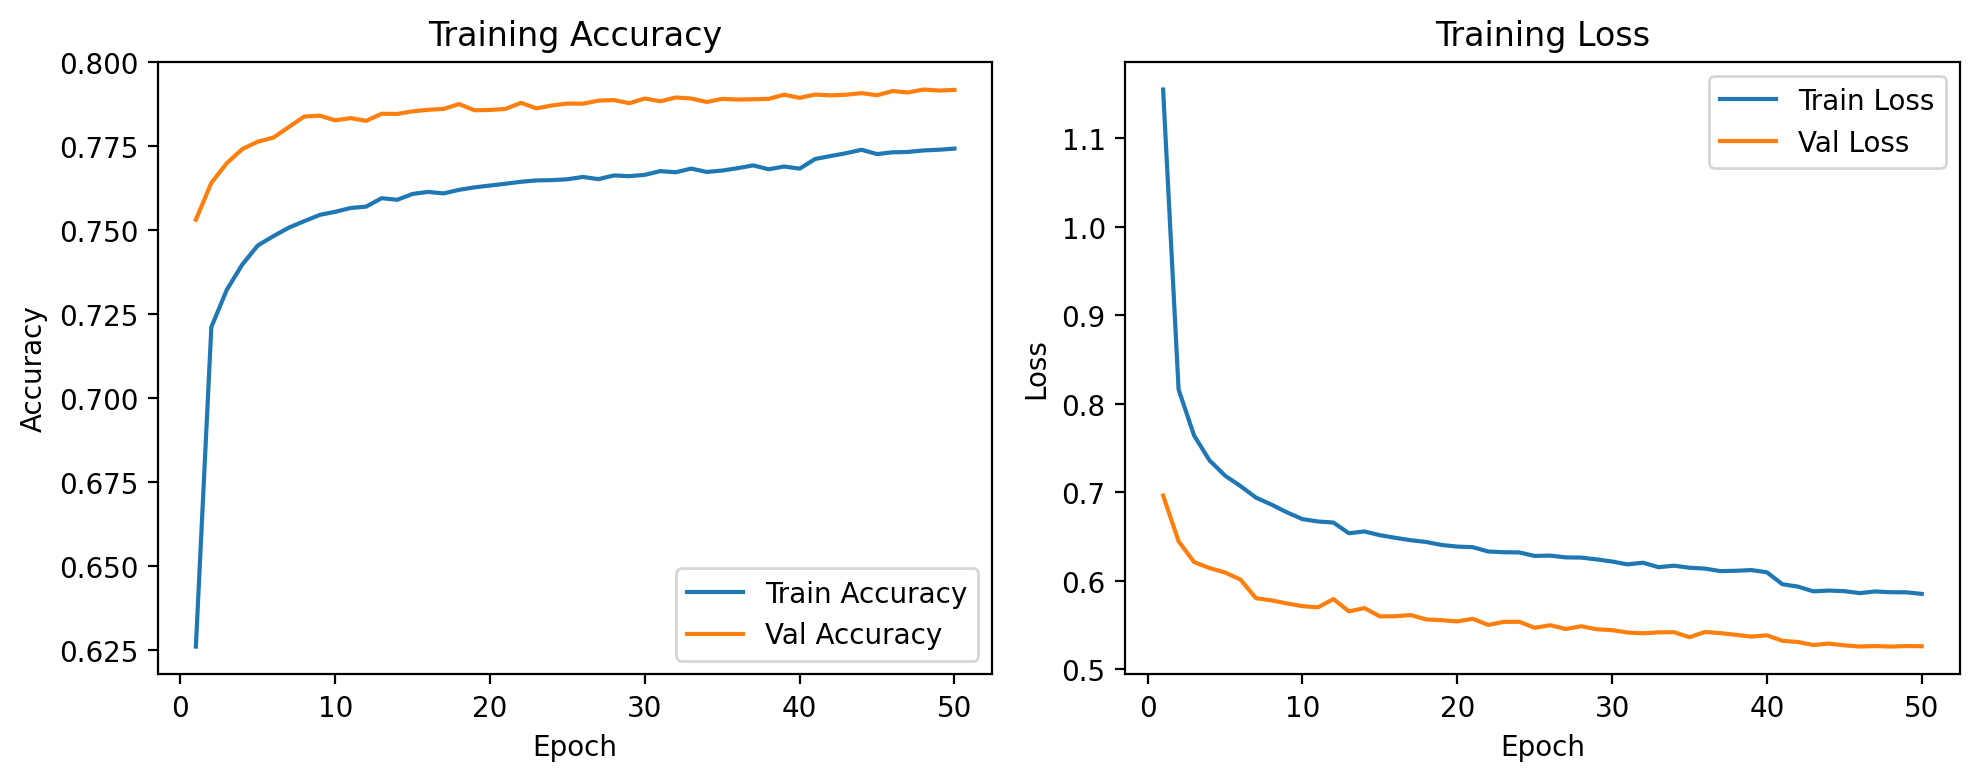
\includegraphics[width=0.4\textwidth]{figs/training_history.png}
	\caption{Graficas de entrenamiento, el de la izquierda mide el porcentaje de aciertos por epoch y el de la derecha cuan lejos se queda de la solución correcta en cada epoch.}
	\label{f:vistageneral}
\end{figure}

Podemos aplicar PCA para reducir la dimensionalidad. Podremos afinar la accuracy modificando la estructura de la red neuronal.





%\begin{table}[!ht]
%\centering
%\begin{tabular}{lccccc}
% x & sin(x) &	cos(x)& tan(x) &  sec(x) & cosec(x)\\
%\hline
%30$^\circ$ & 0.5000 & 0.8660 & 0.5774 & 1.1547 & 2.0000\\
%45$^\circ$ & 0.7071 & 0.7071 & 1.0000 & 1.4142 & 1.4142\\
%60$^\circ$ & 0.8660 & 0.5000 & 1.7321 & 2.0000 & 1.1547\\
%\hline
%\end{tabular}
%\caption{ Raons trigonomètriques per diferents valors d’angles.}
%\label{t:raonstrigonometriques}
%\end{table}

\section{Conclusiones}

Aliquam erat volutpat. Pellentesque habitant morbi tristi-que senectus et netus et malesuada fames ac turpis egestas. Donec ut sapien nec turpis placerat maximus. Quisque port-titor nulla ex, vel finibus nisi commodo in. Vivamus fringilla diam eget est egestas, id hendrerit leo tincidunt. Mauris tin-cidunt iaculis ornare. Curabitur pulvinar, dolor amet ultrices porttitor, odio nisl tincidunt magna, sed dapibus elit tellus vel mauris. Proin faucibus scelerisque orci vitae aliquet. Nulla ullamcorper tincidunt nisl, sit amet mollis mi pretium sit amet. Fusce sagittis vehicula nibh, ut pulvinar magna ves-tibulum eget. Praesent vulputate accumsan eros sed portti-tor. 

Quisque consectetur justo a mi porta, id varius nisi posue-re. Morbi tristique orci nec dolor aliquet venenatis. Integer malesuada tincidunt dignissim. Cras lobortis metus tristique erat placerat, nec rutrum justo pretium. Integer faucibus aliquet commodo. Integer non quam nec lectus. Sed in leo rhoncus, gravida elit vel, tristique quam. Nullam auctor mi in tortor mollis ullamcorper. 

Nunc dictum ipsum quis egestas scelerisque. Vestibulum rutrum tempor posuere. Praesent varius libero odio, ac bibe-ndum arcu tempus quis. Pellentesque habitant morbi tristi-que senectus et netus et malesuada fames ac turpis egestas. Sed eget ex risus. Integer metus velit, viverra ac fringilla sit amet, laoreet eget lacus. Nulla rutrum mollis elit et maximus. Nulla sed aliquet elit. Sed libero justo, porta ut vulputate eget, suscipit faucibus sem. Sed at quam ut justo vestibulum vehicula non sed ligula. 

Nulla facilisi. Curabitur pulvinar, dolor amet ultrices porttitor, odio nisl tincidunt magna, cras lobortis metus tristique erat placerat, sed dapibus elit tellus vel mauris. Phasellus vitae purus gravida, rutrum ante vel, vestibulum mauris. 


\begin{thebibliography}{9}
\bibitem{Techniques2020} M. Oudah, A. Al-Naji, J. Chahl. (23 de Julio de 2020). \newblock ``Hand Gesture Recognition Based on Computer Vision: A Review of Techniques''. \newblock \url{https://pmc.ncbi.nlm.nih.gov/articles/PMC8321080/}
\bibitem{Skeleton2016} Q. De Smedt, H. Wannous and J. -P. Vandeborre. \newblock ``Skeleton-Based Dynamic Hand Gesture Recognition,'' \newblock 2016 IEEE Conference on Computer Vision and Pattern Recognition Workshops (CVPRW), Las Vegas, NV, USA, 2016, pp. 1206-1214, doi: 10.1109/CVPRW.2016.153. keywords: {Gesture recognition;Three-dimensional displays;Skeleton;Shape;Cameras;Sensors;Databases}
\bibitem{dataset_MNIST_ASL} P. Tecle. (2017). \newblock ``Sign Language MNIST Dataset''. \newblock Kaggle Datasets. \newblock \url{https://www.kaggle.com/datasets/datamunge/sign-language-mnist}
\bibitem{dataset_Multi-Modal} GTI-UPM Group. (2019). \newblock ``Multi-modal Hand Gesture Recognition Dataset''. \newblock Kaggle Datasets. \newblock \url{https://www.kaggle.com/datasets/gti-upm/multimodhandgestrec}
\bibitem{IJECE2023} Rifa Tasfia. (2023). \newblock ``Article from International Journal of Electrical and Computer Engineering''. \newblock \url{https://ijece.iaescore.com/index.php/IJECE/article/view/34455/17578}
\bibitem{git} Github del repositorio. \url{https://github.com/Gonzalo-UAB/PSIV_PROYECTO}
\end{thebibliography}
\end{document}

